\section{Controle de vers\~ao}
\subsection{Git}
O GIT é um sistema de controle de versão, de código aberto, tendo como um dos desenvolvedores o conhecido Linus Torvalds.
\begin{quote}
Eu sou um egoísta degenerado, batizo todos os meus projetos com meu nome. Primeiro Linux, agora Git.
— Linus Torvalds
\end{quote}
Lembrando que Git é um gíria para cabeça dura, contudo podendo ter outros sinônimos como: Global information tracker, ou, quando ele trava, ``Goddamn idiotic truckload of sh*t".

\begin{center}
\center
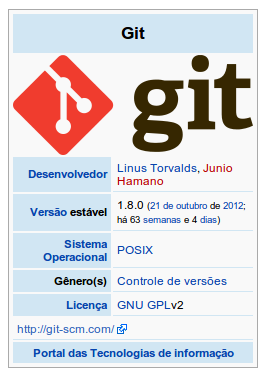
\includegraphics[width=6cm]{./include/chapters/sections/soft/section1/img/git.png}
\label{git wiki}
\end{center}

Uma ferramente de controle de versão possui uma série de periféricos para possibilitar sua utilização, nesta parte iremos introduzir algumas delas.

\begin{enumerate}
\item Criando \\
Para criar um repositório local: git init\\
Para clonar um repositório remoto: git clone  /caminho/para/o/repositório\\
Para clonar um repositório remoto: git clone username@host:/caminho/para/o/repositório ou git clone\\ https://github.com/username/repositório.git\\

\item Adicionando e removendo \\
Para adicionar arquivos no repositório a ser verificado: git add nome\_do\_arquivo
Para adicionar tudo ao repositório: git add *
Para remover um arquivo do repositório: git rm nome\_do\_arquivo

\item Commit (comentar as mudanças) e sincronizar \\
Commitar mudanças: git commit -m ``mensagem de commit"\\
Atualizar o seu repositório: git pull\\
Atualizar o repositório remoto: git push\\
Conectar repositório local com um remoto: git remote add origin server\\

\item Branches (ramos no repositório) \\
Criar um novo branche: git checkout -b nome\_do\_branch\\
Trocar do branch para o master: git checkout master\\
Deletar branch: git branch -d nome\_do\_branch\\
Dar um push do branch para o repositório local: git push origin branch\\

\item Merges (incorporar mudanças) \\
Merge as mudanças de algum branch: git merge nome\_do\_branch\\
Vê as mudanças entre dois branches: git diff branch\_fonte branch\_alvo\\

\end{enumerate}

\begin{figure}[!htb]
\centering
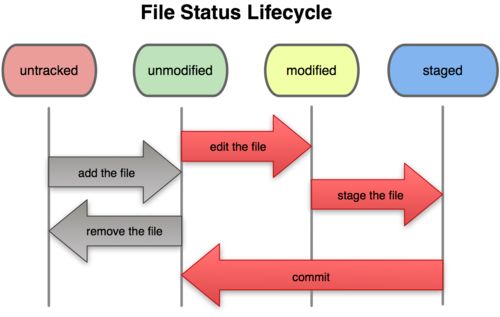
\includegraphics[width=11cm]{./include/chapters/sections/soft/section1/img/filestatus.png}
\caption{Ciclo GIT}
\label{CicloVidaGit}
\end{figure}

A figura \ref{CicloVidaGit}, mostra numa vis\~ao muito simplificada a utiliza\c{c}\~ao do git. \\
Tendo como in\'icio, o arquivo n\~ao rastreado, ``untracked", temos que iniciar o mesmo no reposit\'orio, para isso utilizando o comando: \\ \$ git add nome\_do\_arquivo, \$ git add * ou at\'e mesmo \$ git add $--$all. \\ \\
Tendo em m\~aos o arquivo modificado, organize e comente o mesmo para o commit, fazendo assim uma atualiza\c{c}\~ao do arquivo para o gerenciador de vers\~ao, desta forma o arquivo ira constar como atualizado na sua maquina para ultima vers\~ao, desta forma, basta utilizar o seguinte comando:\\ \$ git commit -m ``mensagem", \$ git commit e escrever a mensagem em seguida.\\ \\
Fazendo tudo isso na sua maquina e tendo o arquivo como n\~ao modificado, ``unmodified", est\'a na de atualizar o servidor remoto, utilizando desta forma o comando: \\
\$ git push origin master \\ \\


\subsection{Primeiros passos}
\begin{enumerate}
\item Configurando.\\
Após a instalação do git.\\
Vamos fazer algumas configurações do usuario. \\
username:   \\
\$ git config --global user.name ``seu nome"  \\
Email:      \\
\$ git config --global user.name ``seu\_mail@exemplo.com" \\

Esses dados são uteis, pois iram junto com seus commits.\\
Caso esteja utilizando o GitHub, é altamente aconselhável utilizar o mesmo e-mail para ambos.\\
Pode visualizar as modificações utilizando:\\
\$ git config --list

\item Conseguindo um repositório git.\\

a) Inicializando um repositório de um diretório existente.\\
\$ git init \\
Este comando cria um subdiretório .git, que ira conter todos os arquivos necessários para o git.\\
Após isso é necessário adicionar os arquivos que você gostaria de serem adicionados ao nosso repositório.\\
\$ git add README		\\
Após adicionar nossos arquivos, vamos agora comentar as modificações.\\
\$ git commit -m ``primeiro commit, adicionado os arquivos"\\
Terminando isso seu repositório Git esta pronto e atualizado, podendo ser visualizado pelo comando:\\
\$ gitk\\

b) Iniciando um repositório utilizando um existente.\\
Em sua essência utilizamos o comando:\\
\$ git clone url \\
Que, por sua vez, clona um repositório ja existente.\\
Ex: \$ git clone git://github.com/live/4ever.git\\
Como o ``\$ git init" ele também cria uma pasta .git que possui todo o  histórico e modificações do repositório.

\item Salvando modificações.\\
Para checar o status dos arquivos, utilizamos o comando:\\
\$ git status \\
Se o retorno for: nothing to commit (working directory clean),significa que seu repositório esta atualizado.\\
Caso for diferente, devemos atualizar o repositório e comentar as mudanças.\\
Para rastrear arquivos dentro do diretório, utilizamos o comando:\\
\$ git add \\
Caso todos os arquivos dentro da pasta estejam no diretório, é recomendado utilizar:\\
\$ git add --all\\
Arquivos específicos:\\
\$ git add README\\
Arquivos com extensão especifica:\\
\$ git add *.c\\

Para poder ver a situação atual do repositório utilizando o comando status do Git, ``\$ git status", 
permitindo desta forma visualizar modificaç\~oes depois do ultimo commit.
Utilizando o comando de status, poderemos ver:\\

Algumas extensões são ignoradas pelo comando ``\$ git add", geralmente são arquivos de compilação e temporários:\\
*.o\\
*.a\\
*$\sim$\\

Visualizando modificações.\\
A principal ferramenta para visualizar as modificações do ultimo commit é o comando ``\$ git diff", mostra os arquivos e linhas modificadas. A visualização é bem instintiva e de grande ajuda para os commits realizados no futuro.\\

Commitando as modificações.\\
Após adicionar o arquivo e modificar, vamos agora commitar as modificações, esta ação atualiza todos os arquivos rastreados pelo git,fazendo dessa forma um update do repositório local comentado.\\
O comando base:\\
\$ git commit\\
(Este comando utiliza da variável Shell \$EDITOR, vim,emacs,nano. Caso não esteja configurado no seu OS, utilize o comando ``\$ git config --global core.editor").

Abrindo tela, é possível deixar uma mensagem para comentar as atualizações.\\
Para tornar este comando mais pratico, existe a possibilidade de adicionar a variável -m.\\
Ex: \$ git commit -m ``o arquivo README foi modificado"\\

\item Visualizando o histórico do commit.\\

Após dar um clone num repositório, podemos visualizar todas os commits realizados durante sua existência utilizando o comando ``\$ git log".\\
Esta função do git, possui inúmeras funcionalidades e variáveis para ajudar o desenvolvedor, contudo existi uma ferramenta mais amigável:\\
\$ gitk\\
\begin{figure}[!htb]
\centering
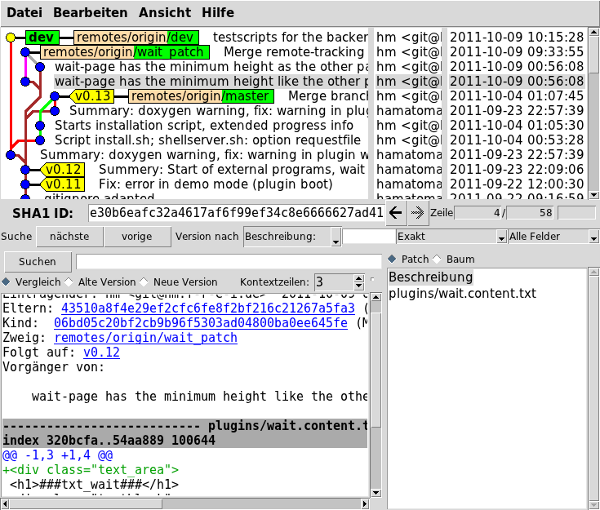
\includegraphics[width=11cm]{./include/chapters/sections/soft/section1/img/gitk.png}
\caption{Gitk}
\label{Gitk}
\end{figure}

\item Trabalhando com um repositório remoto.

Trabalhando num repositório remoto, abre as portas para novas oportunidades e colaboração entre os desenvolvedores.\\
Primeiramente, vamos clonar um repositório:\\
\$ git clone url\\
Este comando permite fazer uma c\'opia do reposit\'orio remoto para seu computador.\\
Você também pode adicionar a variável -v,podendo mostrar a url que foi retirada o repositório.\\
\$ git remote -v

Atualizando o repositório remoto.\\
Caso seu repositório local esta pronto, podemos enviar as modificações para o servidor remoto, utilizando o comando:\\
\$ git push origin master\\
(Tendo previamente definido.)\\

\item Marcações.\\

Utilizado geralmente para marcar a versão que estamos trabalhando no projeto (v1.0 e assim por diante), vamos agora dar alguns exemplos.\\
A listagem das tags pode ser feita utilizando o comando:\\
\$ git tag\\
\# v0.1 \\
\# v1.3\\
Este comando lista as marcas em ordem alfabética, a ordem em  que eles aparecem não possui nenhuma importância.

Criando Marcações.\\
Pode ser feito marcações (-a) com comentários (-m):\\
\$ git tag -a v1.4 -m 'minha versão 1.4'\\
\$ git tag\\
\# v0.1\\
\# v1.3\\
\# v1.4\\

Você pode visualizar as informações da marcação, com o comando:\\
\$ git tag show v1.4\\
\# tag v1.4\\
\# Tagger: Scott Chacon schacon@gee-mail.com\\
\# Date:   Mon Feb 9 14:45:11 2009 -0800\\
\# \\
\# my version 1.4\\
\# commit 15027957951b64cf874c3557a0f3547bd83b3ff6\\
\# Merge: 4a447f7... a6b4c97...\\
\# Author: Scott Chacon schacon@gee-mail.com\\
\# Date:   Sun Feb 8 19:02:46 2009 -0800\\
\# \\
\#     Merge branch 'experiment'\\
\# \\

Pode ser feita uma pesquisa rápida e limitada.\\
\$ git tag-l 'v1.4.2. *' \\
\# v1.4.2.1 \\
\# v1.4.2.2 \\
\# v1.4.2.3 \\
\# v1.4.2.4\\

Compartilhando marcações.\\
Por padrão o comando ``\$ git push" não transfere tags para servidores remotos.\\
A maneira existente para fazer isso, seria utilizar o comando no formato:\\
\$ git push origin nome\_da\_tag\\
Ex: \$ git push origin v1.5\\
\# Counting objects: 50, done.\\
\# Compressing objects: 100\% (38/38), done.\\
\# Writing objects: 100\% (44/44), 4.56 KiB, done.\\
\# Total 44 (delta 18), reused 8 (delta 1)\\
\# To git@github.com:schacon/simplegit.git\\
\# * [new tag]         v1.5 - v1.5\\

Se existe um numero grande de marcações que gostaria de dar push, pode utilizar --tags como opção.\\
\$ git push origin --tags\\
\# Counting objects: 50, done.\\
\# Compressing objects: 100\% (38/38), done.\\
\# Writing objects: 100\% (44/44), 4.56 KiB, done.\\
\# Total 44 (delta 18), reused 8 (delta 1)\\
\# To git@github.com:schacon/simplegit.git\\
\#  * [new tag]         v0.1 - v0.1\\
\#  * [new tag]         v1.2 - v1.2\\
\#  * [new tag]         v1.4 - v1.4\\
\#  * [new tag]         v1.5 - v1.5\\
\end{enumerate}

\subsection{Ramificações ou Branchs}

O Branch pode ser simplesmente definido como:
\begin{quote}
Um branch no Git é simplesmente um leve ponteiro móvel para um desses commits. O nome do branch padrão no Git é master. Como você inicialmente fez commits, você tem um branch principal (master branch) que aponta para o último commit que você fez. Cada vez que você faz um commit ele avança automaticamente. 
— \href{http://git-scm.com/book/pt-br/Ramifica\%C3\%A7\%C3\%A3o-Branching-no-Git-O-que-\%C3\%A9-um-Branch}{git-scm}
\end{quote}

A figura \ref{Branch} exemplifica como funciona na pratica, o branch da inicio no ultimo commit e quando terminado o objetivo dele, as modificações são aplicadas ao master.

\begin{figure}[!htb]
\centering
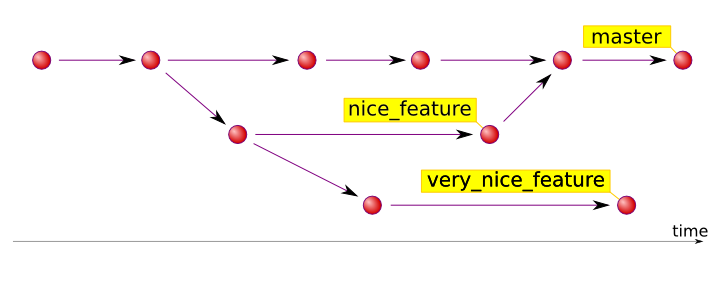
\includegraphics[width=11cm]{./include/chapters/sections/soft/section1/img/branch.png}
\caption{Exemplo de Branch}
\label{Branch}
\end{figure}

Para criar um Branch basta utilizar o comando:\\
\$ git checkout -b  nome\_do\_branch\\
\$ git branch  nome\_do\_branch\\
Ex: \$ git checkout -b nice\_feature\\
Ex: \$ git branch nice\_feature\\

Para nosso diret\'orio apontar para o novo branch, devemos utilizar o comando:\\
\$ git checkout nome\_do\_branch\\
Ex:\$ git checkout nice\_feature\\

Como pode ser visto na figura \ref{checkout}, podemos ver que com o checkout mudamos o local do ponteiro onde estamos trabalhando, desta forma, as modificaç\~oes serão feitas aonde o apontador esta localizado.

\begin{figure}[!htb]
\centering
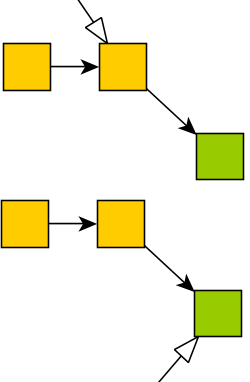
\includegraphics[width=4cm]{./include/chapters/sections/soft/section1/img/apontador3.png}
\caption{Exemplo checkout}
\label{checkout}
\end{figure}
Ap\'os as modificaç\~oes serem realizadas, esta na hora de integrar as modificaç\~oes com o branch master.\\

Primeiramente, devemos estar com o nosso apontador no master:\\
\$ git checkout master\\
Em seguida, fazer o merge e atualizar nosso master com a nice\_feature:\\
\$ git merge - -no-ff nice\_feature\\
\# Merge made by recursive.\\
\# README | 1 +\\
\# 1 files changed, 1 insertions(+), 0 deletions(-)\\

É recomendado que utilize o comando ``\$ git merge - -no-ff nice\_feature" com a opção - -no-ff, pois:
\begin{quote}
Isso evita a perda de informações sobre a existência histórica de um ramo e suas características, junto com todos os commits.
— \href{http://nvie.com/posts/a-successful-git-branching-model/}{nvie}
\end{quote}

A figura \ref{noff} exemplifica bem a diferença.\\
\begin{figure}[!htb]
\centering
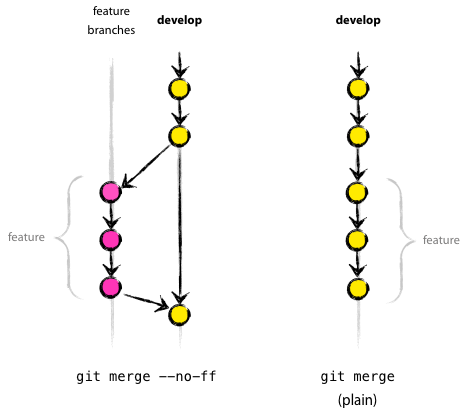
\includegraphics[width=9cm]{./include/chapters/sections/soft/section1/img/off.png}
\caption{Exemplo da opç\~ao - -no-ff}
\label{noff}
\end{figure}

Com a atualização do seu master, não existe mais a necessidade de ter ainda em paralelo o branch,
assim podemos deletar o mesmo, utilizando o comando:\\
\$ git branch -d nome\_do\_branch\\
Ex: \$ git branch -d nice\_feature\\

Conflitos de Merge.

Como visto na figura \ref{checkout}, temos em paralelo o branch nice\_feature com o branch very\_nice\_feature.
Contudo, pode acontecer alguns problemas, se for alterada a mesma parte do mesmo arquivo de forma diferente nos dois branches, o Git não será capaz de executar o merge  de forma clara, o conflito pode ser demostrado com:\\
\$ git merge very\_nice\_feature\\
\# Auto-merging index.html\\
\# CONFLICT (content): Merge conflict in index.html\\
\# Automatic merge failed; fix conflicts and then commit the result.\\

Todo conflito de merge que não foi resolvido é listado como ``unmerged" no comando ``\$ git status" no branch master.\\
\$ git status\\
\# index.html: needs merge\\
\# On branch master\\
\# Changes not staged for commit:\\
\#   (use "git add file..." to update what will be committed)\\
\#   (use "git checkout -- file ..." to discard changes in working directory)\\
\#\\
\#    unmerged:   index.html\\
\#\\

Gerenciamento de Branch.

Para ter uma lista de branchs existentes no repositório, é possível utilizar o comando:\\
\$ git branch\\
\#   nice\_feature\\
\# * master\\
\#   very\_nice\_feature\\
O simbolo \* mostra aonde o apontador est'\a localizado.\\
Para ver o \'ultimo commit feito em cada branch, pode ser executado o comando:\\
\$ git branch -v
%contribuindo para o projeto talvez nova sub de projeto, criar um para o robota ?
%http://git-scm.com/book/pt-br/Git-Distribu%C3%ADdo-Contribuindo-Para-Um-Projeto

